\subsection{Prototyping og produksjon}
\label{sec:prototyping}
De fysiske delene utvikles i fire serier etter metoden i seksjon~\ref{sec:iterativ-prototyping}: lagersete (LS), feste av nav på aksel (NV), snortrommel (TR) og drivhjul med dekk (DH). Alle bygger på DV-3 fra seksjon~\ref{sec:dv-serien}. Figur~\ref{fig:prototype} viser prototypen slik den er brukt i utsnurringstestene, med den generative rammen fra seksjon~\ref{sec:gd-ramme}, svinghjul, tannhjulspar og måleoppsett.

\begin{figure}[H]
    \centering
    \begin{subfigure}[b]{0.56\textwidth}
        \centering
        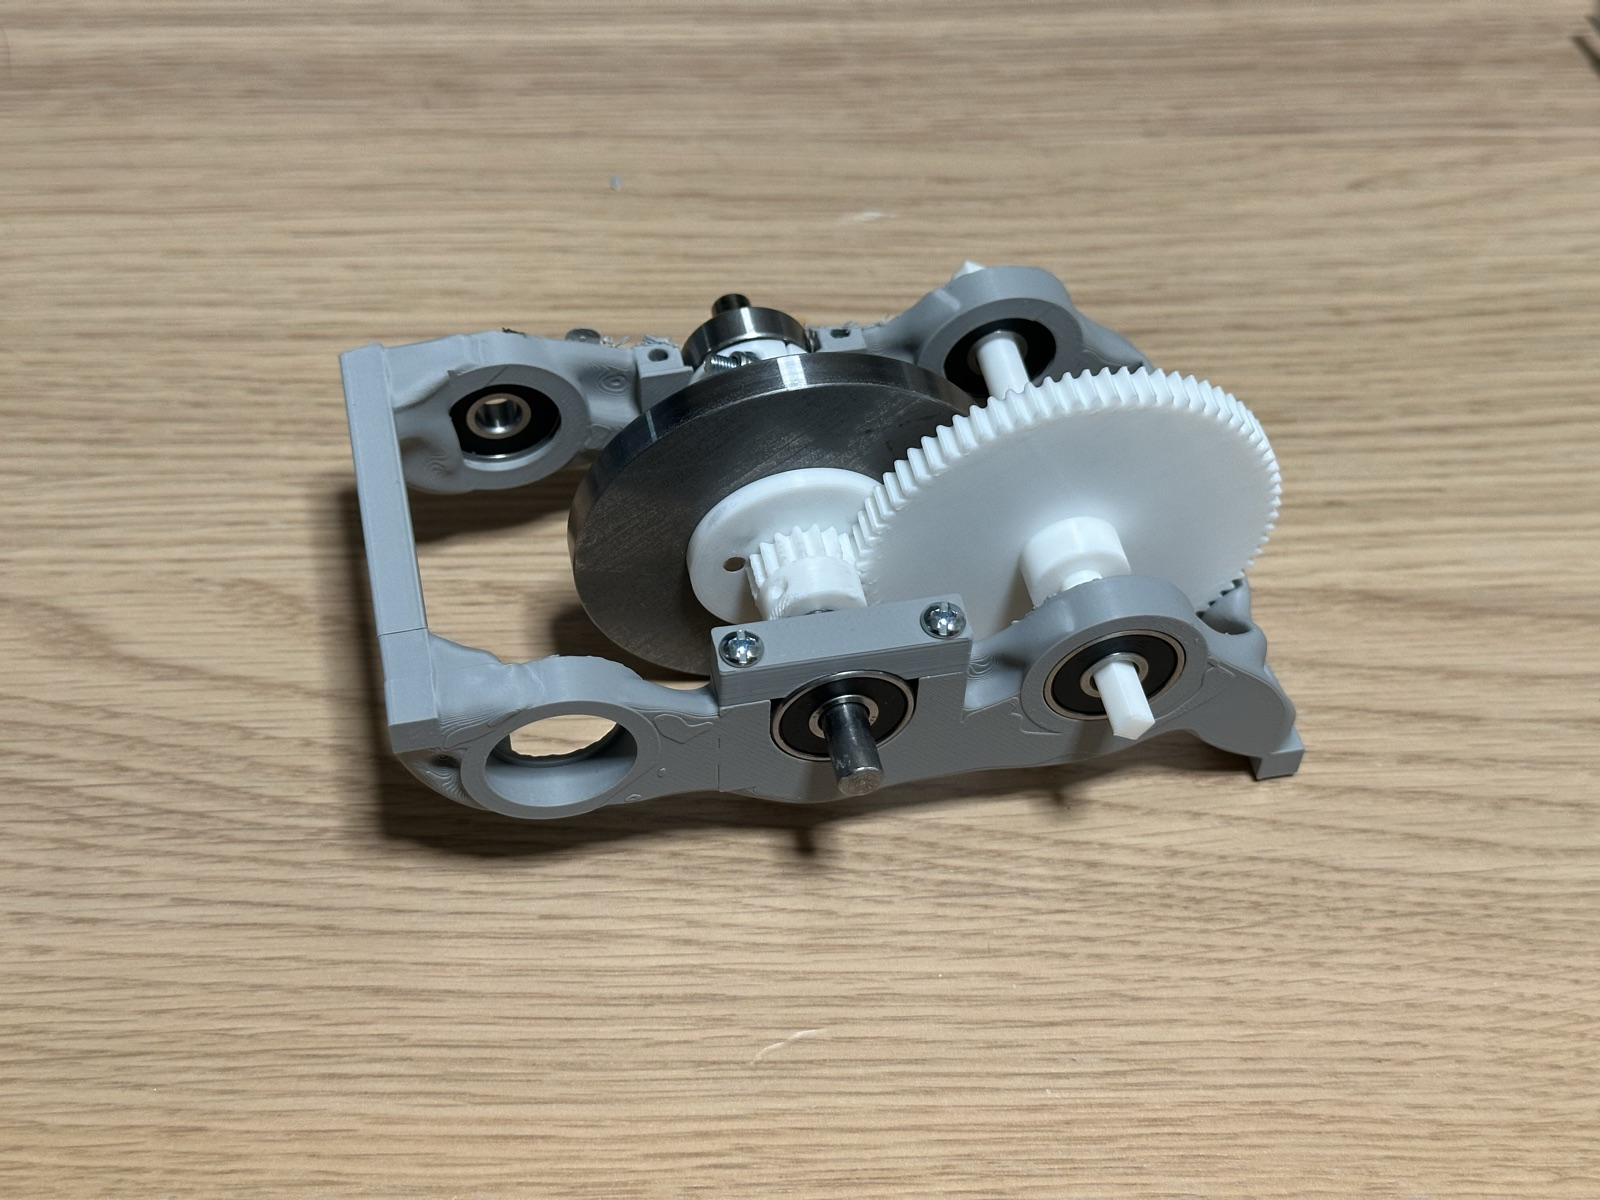
\includegraphics[width=\textwidth]{Images/Foto/prototype_skraatt.jpg}
        \caption{Skrått forfra}
    \end{subfigure}
    \hspace{1.5em}
    \begin{subfigure}[b]{0.315\textwidth}
        \centering
        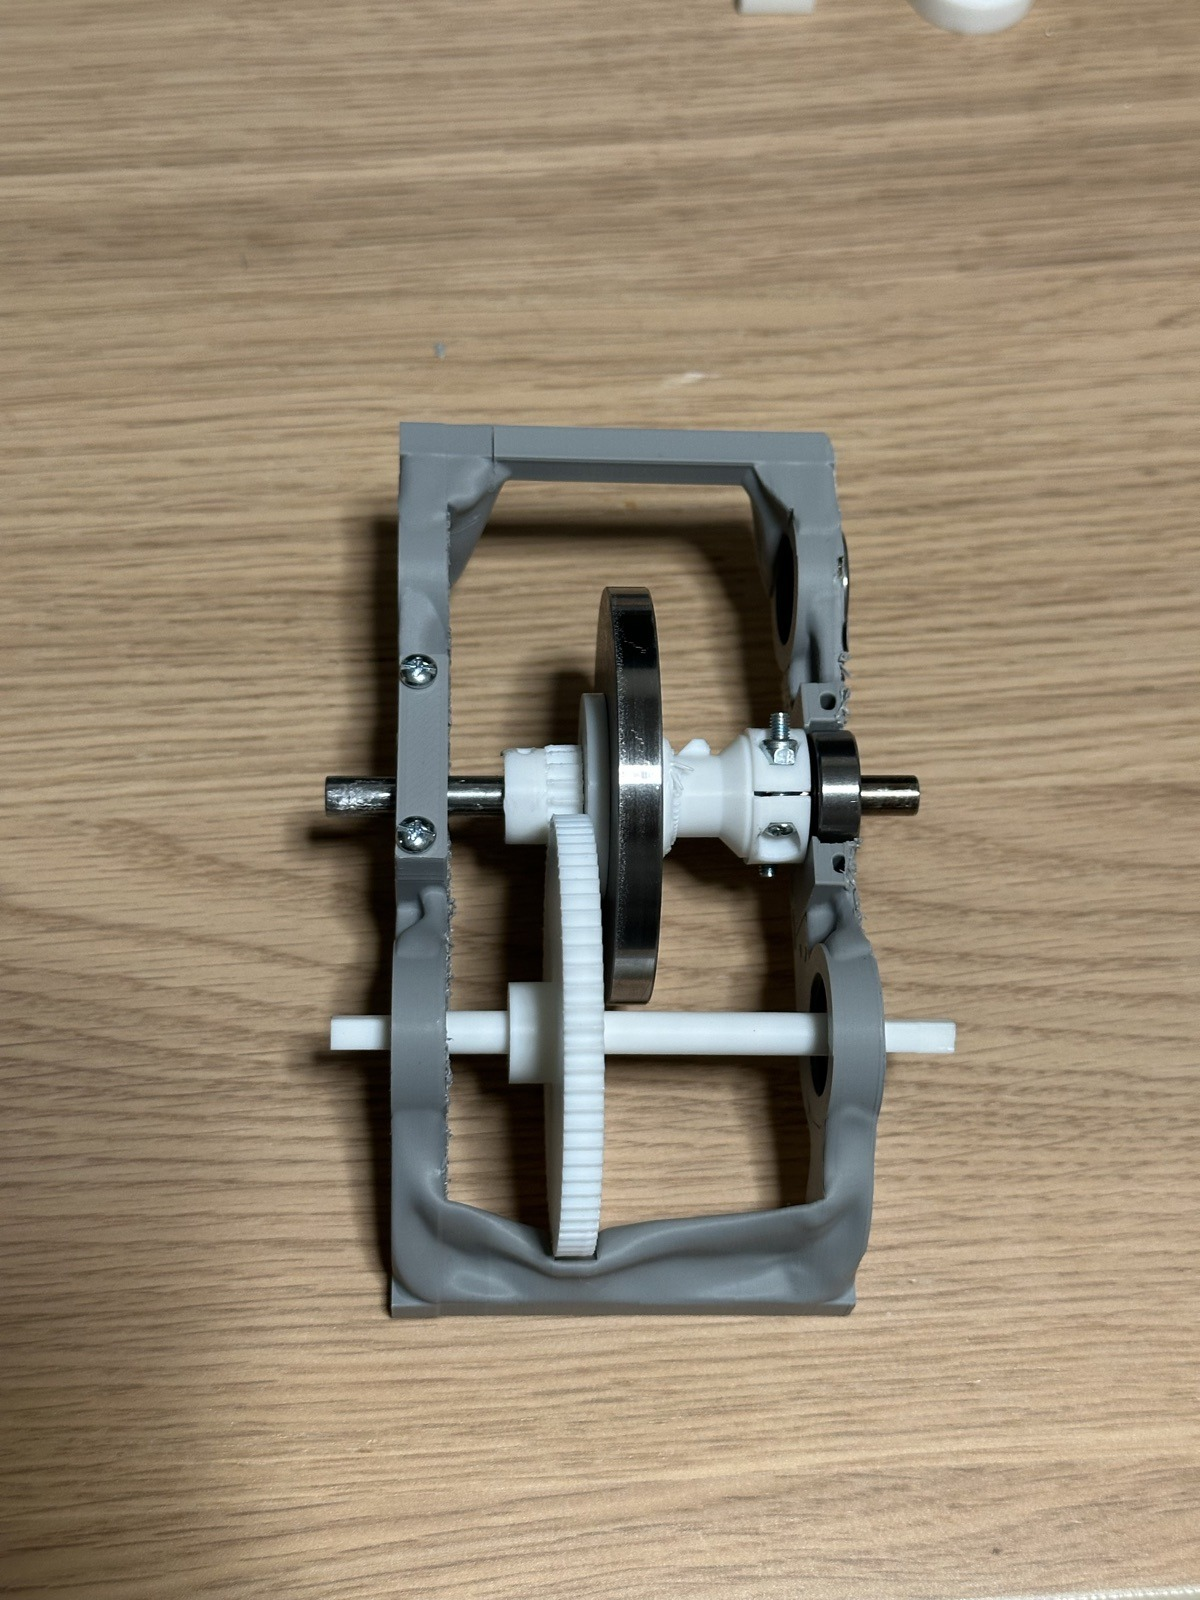
\includegraphics[width=\textwidth]{Images/Foto/prototype_ovenfra.jpg}
        \caption{Ovenfra}
    \end{subfigure}
    \caption{Prototypen med svinghjul, pinjong og tannhjul i den 3D-printede rammen.}
    \label{fig:prototype}
\end{figure}


\subsubsection{Lagersete (LS)}
\label{sec:ls-serien}
De seks 626-lagrene har ytterdiameter \SI{19}{mm} og sitter i rammen. Setet må holde lageret fast uten å klemme det så hardt at det går tungt. \textcite{espedal_2024} fant at hull fra 3D-printer ble 0,5--\SI{0,8}{mm} mindre enn tegnet, så målene på tegningen kan ikke brukes direkte. Serien starter derfor med en prøvebit, LS-0, med lagerseter fra Ø18,8 til Ø19,4 mm i trinn på \SI{0,1}{mm}. Prøvebiten har også glidehull for forakselen fra Ø6,1 til Ø6,5 mm. Den lages med samme produksjonsmetode og innstillinger som sideplatene. Hullene måles med skyvelære, og lageret og akselen prøves i hvert hull. Det hullet som gir best pasning, bestemmer målet i LS-1, som er setet i selve rammen.

Hovedtesten er at lageret sitter fast og går lett (R13). Tilleggstester er at lageret kan tas ut og settes inn igjen uten at setet blir slakt (R10), og at akslene blir parallelle i rammen.

Prøvebiten ble laget som fem ringer fra Ø18,9 til Ø19,3 mm, merket med ett til fem hakk og printet i samme retning som rammen (figur~\ref{fig:lager-proevering}). Ø19,0 gikk inn, men stramt, og Ø19,1 var litt romslig. Ø19,1 er brukt i rammen (seksjon~\ref{sec:gd-ramme}).

\begin{figure}[H]
    \centering
    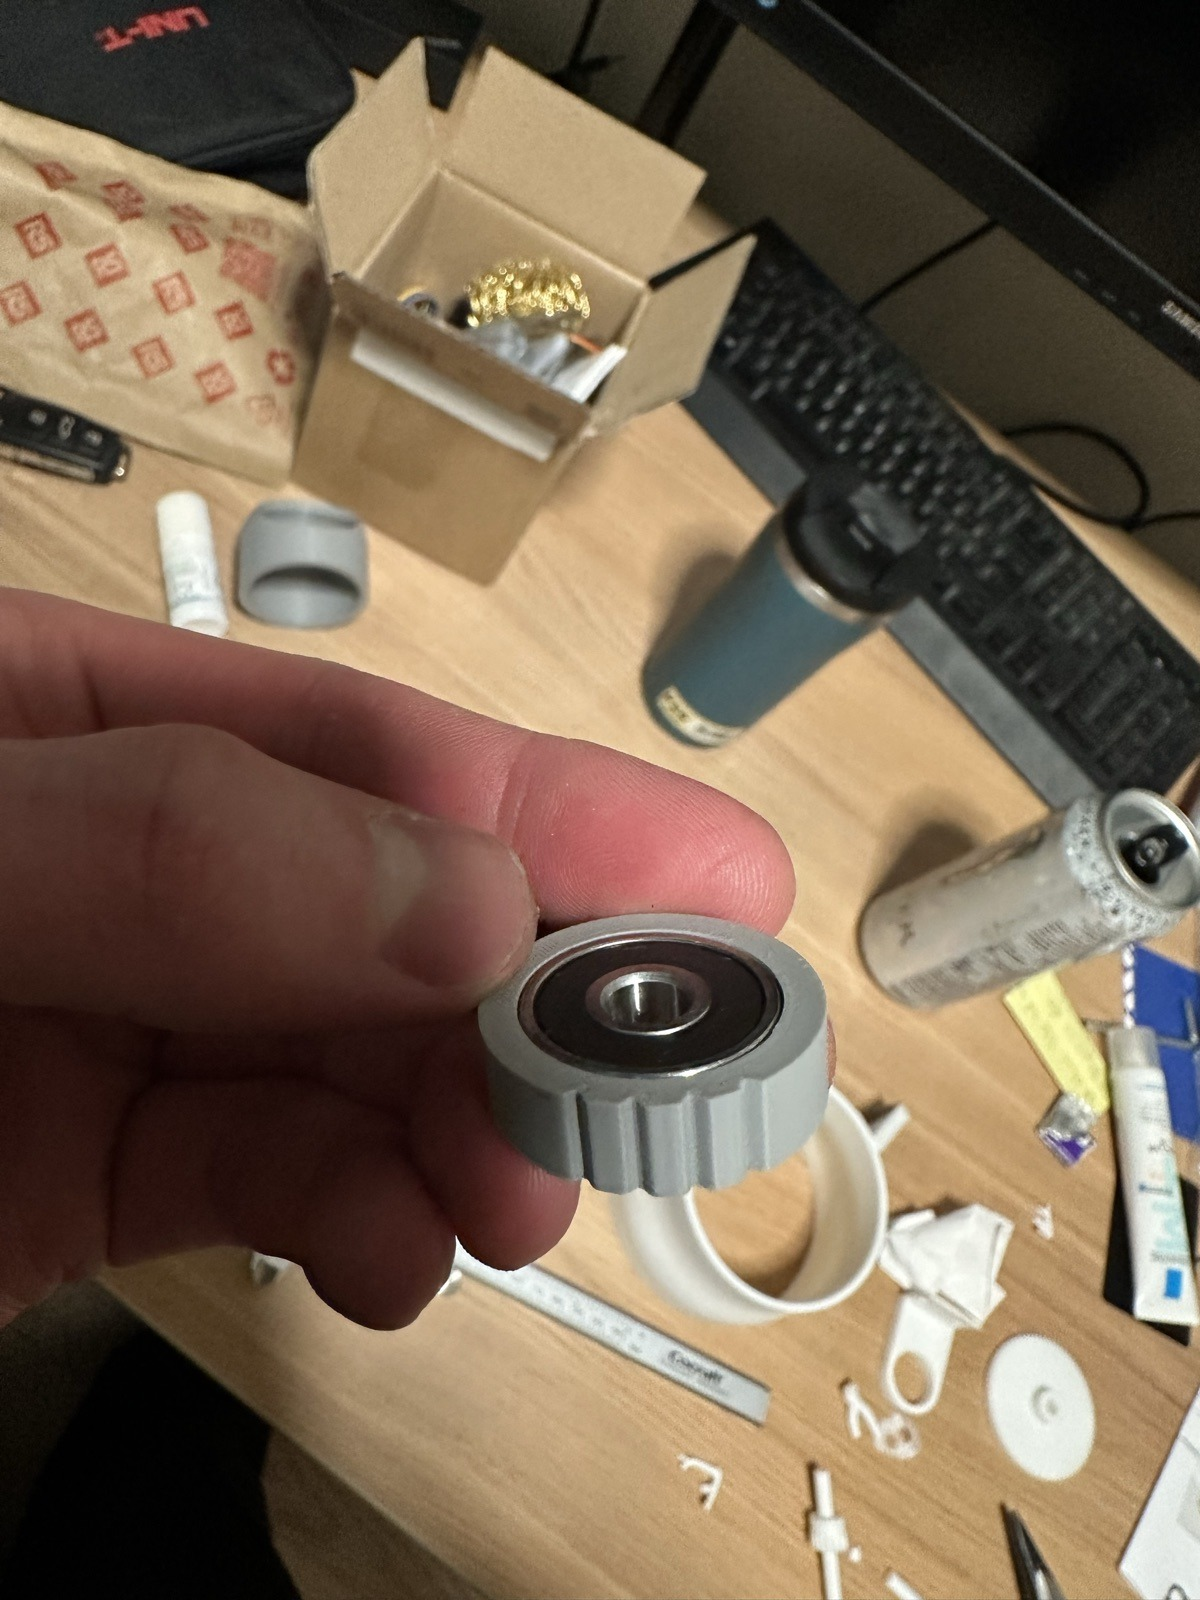
\includegraphics[width=0.33\textwidth]{Images/Foto/lager_proevering.jpg}
    \caption{626-lager i en av prøveringene for lagersetet.}
    \label{fig:lager-proevering}
\end{figure}

\begin{comment}
\begin{table}[H]
    \centering
    \caption{Målt diameter på lagerseter i prøvebiten LS-0}
    \label{tab:ls0-toleranse}
    \small
    \renewcommand{\arraystretch}{1.3}
    \begin{tabular}{|c|c|c|l|}
        \hline
        \textbf{Tegnet [mm]} & \textbf{Målt [mm]} & \textbf{Avvik [mm]} & \textbf{Pasning med lager} \\
        \hline
        18,8 & & & \\
        \hline
        18,9 & & & \\
        \hline
        19,0 & & & \\
        \hline
        19,1 & & & \\
        \hline
        19,2 & & & \\
        \hline
        19,3 & & & \\
        \hline
        19,4 & & & \\
        \hline
    \end{tabular}
\end{table}

\begin{versjonstabell}{LS-1}{tab:ls1}
    \hovedtest
    Lageret sitter fast og går lett (R13) & \\
    \tilleggstester
    Lageret kan tas ut og settes inn igjen (R10) & \\
    Akslene er parallelle etter montering & \\
\end{versjonstabell}
\end{comment}

\subsubsection{Feste av nav på aksel (NV)}
\label{sec:nv-serien}
Pinjongen, tannhjulet, trommelen og hjulene festes til Ø6-akslene. Delene kan ikke ha D-hull, fordi de må tres forbi de runde lagersetene på akselen. Opprinnelig var planen runde Ø6,2-hull med en M3-madenskrue mot en frest flate. Madenskruer var ikke tilgjengelig, mens vanlige M3-skruer og muttere var det, og serien ble lagt om til to festemåter:
\begin{description}
    \item[NV-1: Klemnav.] Brukes på trommelen og pinjongen. Navet er Ø20 med Ø6,2-hull og to slisser på \SI{1}{mm}. To M3 × 12-skruer går på tvers av slissene og strammes mot muttere i sekskantlommer. Skruene står 180° fra hverandre, så navet er balansert. Navet kan løsnes og skyves langs akselen, noe som gjør det mulig å justere delene sideveis (R10).
    \item[NV-2: Firkantnav.] Brukes på hjulene. Akselendene freses til en 4 × 4 mm firkant, med diagonal \SI{5,66}{mm}, mindre enn Ø6. Hjulet tres på firkanten og kan ikke slure.
\end{description}

Firkanthullet ble bestemt med en prøvebit på samme måte som LS-0, med fire hull fra \SI{4,0}{mm} til \SI{4,3}{mm} i trinn på \SI{0,1}{mm}, merket med én til fire streker. Hullet på \SI{4,3}{mm} ga best pasning på den freste akselenden og er brukt i hjulene. Hullene har små avlastningssirkler i hjørnene, så de skarpe hjørnene på den freste firkanten går inn.

\begin{figure}[H]
    \centering
    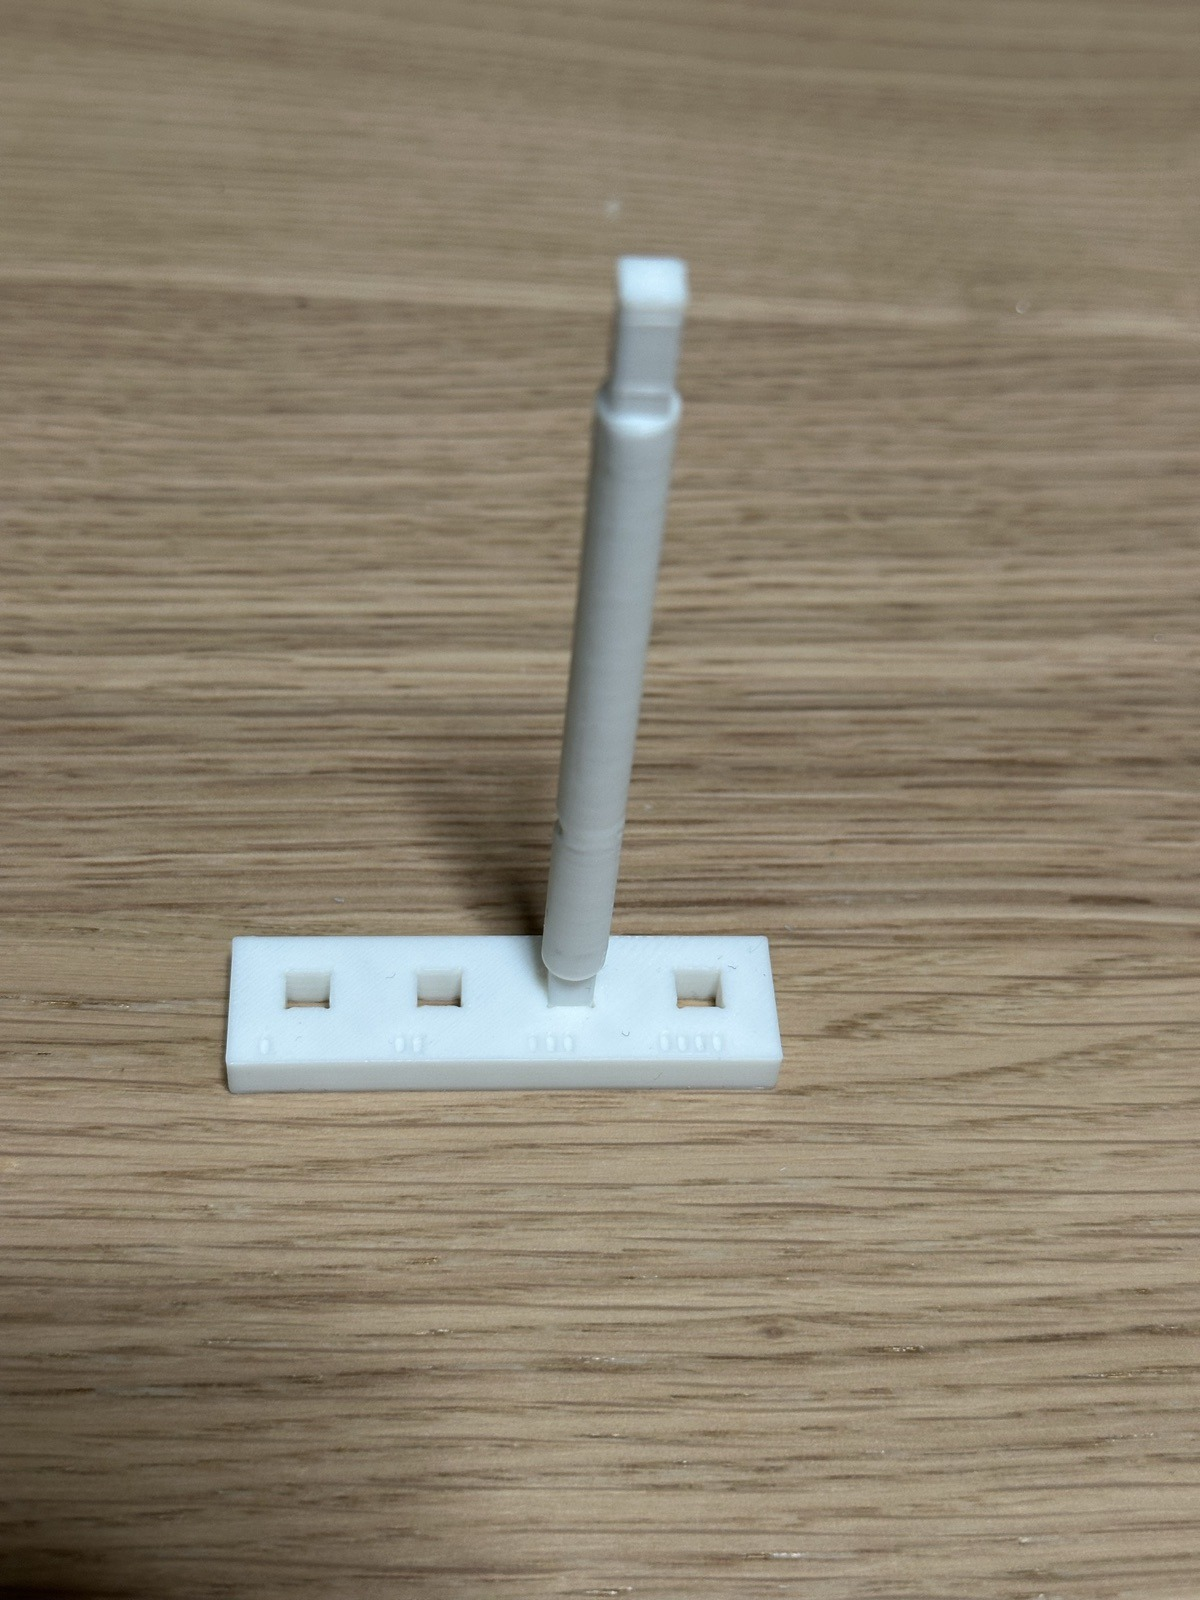
\includegraphics[width=0.36\textwidth]{Images/Foto/firkanttest.jpg}
    \caption{Prøvebiten for firkanthullet. Strekene ved hullene viser størrelsen, fra én strek for \SI{4,0}{mm} til fire for \SI{4,3}{mm}.}
    \label{fig:firkanttest}
\end{figure}

Hovedtesten er at navet ikke slurer på akselen under opptrekk eller når svinghjulet stoppes brått (R9). Tilleggstester er at navet kan demonteres og monteres flere ganger uten at festet blir dårligere (R10), og at skruene ikke løsner i løpet av en testserie.

Under den første utsnurringsserien løsnet klemnavet på trommelen. Trommelen sklei på akselen under opptrekket, og toppturtallet falt fra omtrent 1500 til \SI{1000}{o/min}. Mutterne ble kontrollert og skruene strammet jevnt, og etter det holdt navet gjennom 14 opptrekk i de to neste seriene. Pinjongnavet ble løsnet og flyttet da tannhjulet ble koblet fra (seksjon~\ref{sec:res-utsnurring}), uten at festet ble dårligere.

\begin{versjonstabell}{NV-1}{tab:nv1}
    \hovedtest
    Trommelnavet slurer ikke under opptrekk (R9) & Delvis vellykket, løsnet i første serie, holdt etter ny stramming \\
    \tilleggstester
    Kan demonteres, flyttes og monteres igjen (R10) & Vellykket \\
    Skruene løsner ikke i løpet av en testserie & Delvis vellykket \\
\end{versjonstabell}

\begin{comment}
\begin{versjonstabell}{NV-2}{tab:nv2}
    \hovedtest
    Hjulet slurer ikke på akselen (R9) & \\
    \tilleggstester
    Kan demonteres og monteres flere ganger (R10) & \\
\end{versjonstabell}
\end{comment}

\subsubsection{Snortrommel (TR)}
\label{sec:tr-serien}
Svinghjulet spinnes opp med \SI{20}{cm} snor rundt en trommel på svinghjulsakselen. Ved \SI{4000}{o/min} har svinghjulet energien $E = \frac{1}{2} I \omega^2 \approx \SI{5,3}{J}$. Over \SI{20}{cm} snor tilsvarer det en snittkraft på $E/L \approx \SI{26}{N}$, uavhengig av trommelens diameter. Trommelradien $r_t$ bestemmer derimot hvor fort snora må trekkes, siden $v = \omega r_t$. En mindre trommel gir høyere turtall ved samme trekkhastighet, men kraften som trengs underveis øker. Hypotesen er at én trommeldiameter gir høyest turtall for et opptrekk for hånd.

TR-1 til TR-3 har kjerne med diameter \SI{12}{mm}, \SI{14}{mm} og \SI{18}{mm}, og ellers lik utforming. Figur~\ref{fig:snortrommel} er maskintegningen av TR-1. Snora festes med en løkke på en krok midt i kjernen, utformet som en knaggkrok: en stilk med en finger som peker mot rotasjonsretningen under opptrekket (detalj E). Så lenge snora trekker, holder fingeren løkka på plass. Når snora er trukket helt ut og trommelen spinner videre, snur trekket, og løkka glir av over fingertuppen av seg selv. Undersiden av kroken skrår 45°, så den printes uten support. Den indre flensen har en utsparing for sveisekransen mellom svinghjulet og akselen. Innsiden av den ytre flensen har 45° helning, så trommelen kan printes uten support. Trommelen festes med klemnavet fra NV-1. Magnetene til måleoppsettet sitter ikke i trommelen, men i en egen skive på den andre siden av svinghjulet (seksjon~\ref{sec:ml-serien}). Trommelen veier 3,7 til \SI{6,3}{g}.

\begin{sidewaysfigure}
    \centering
    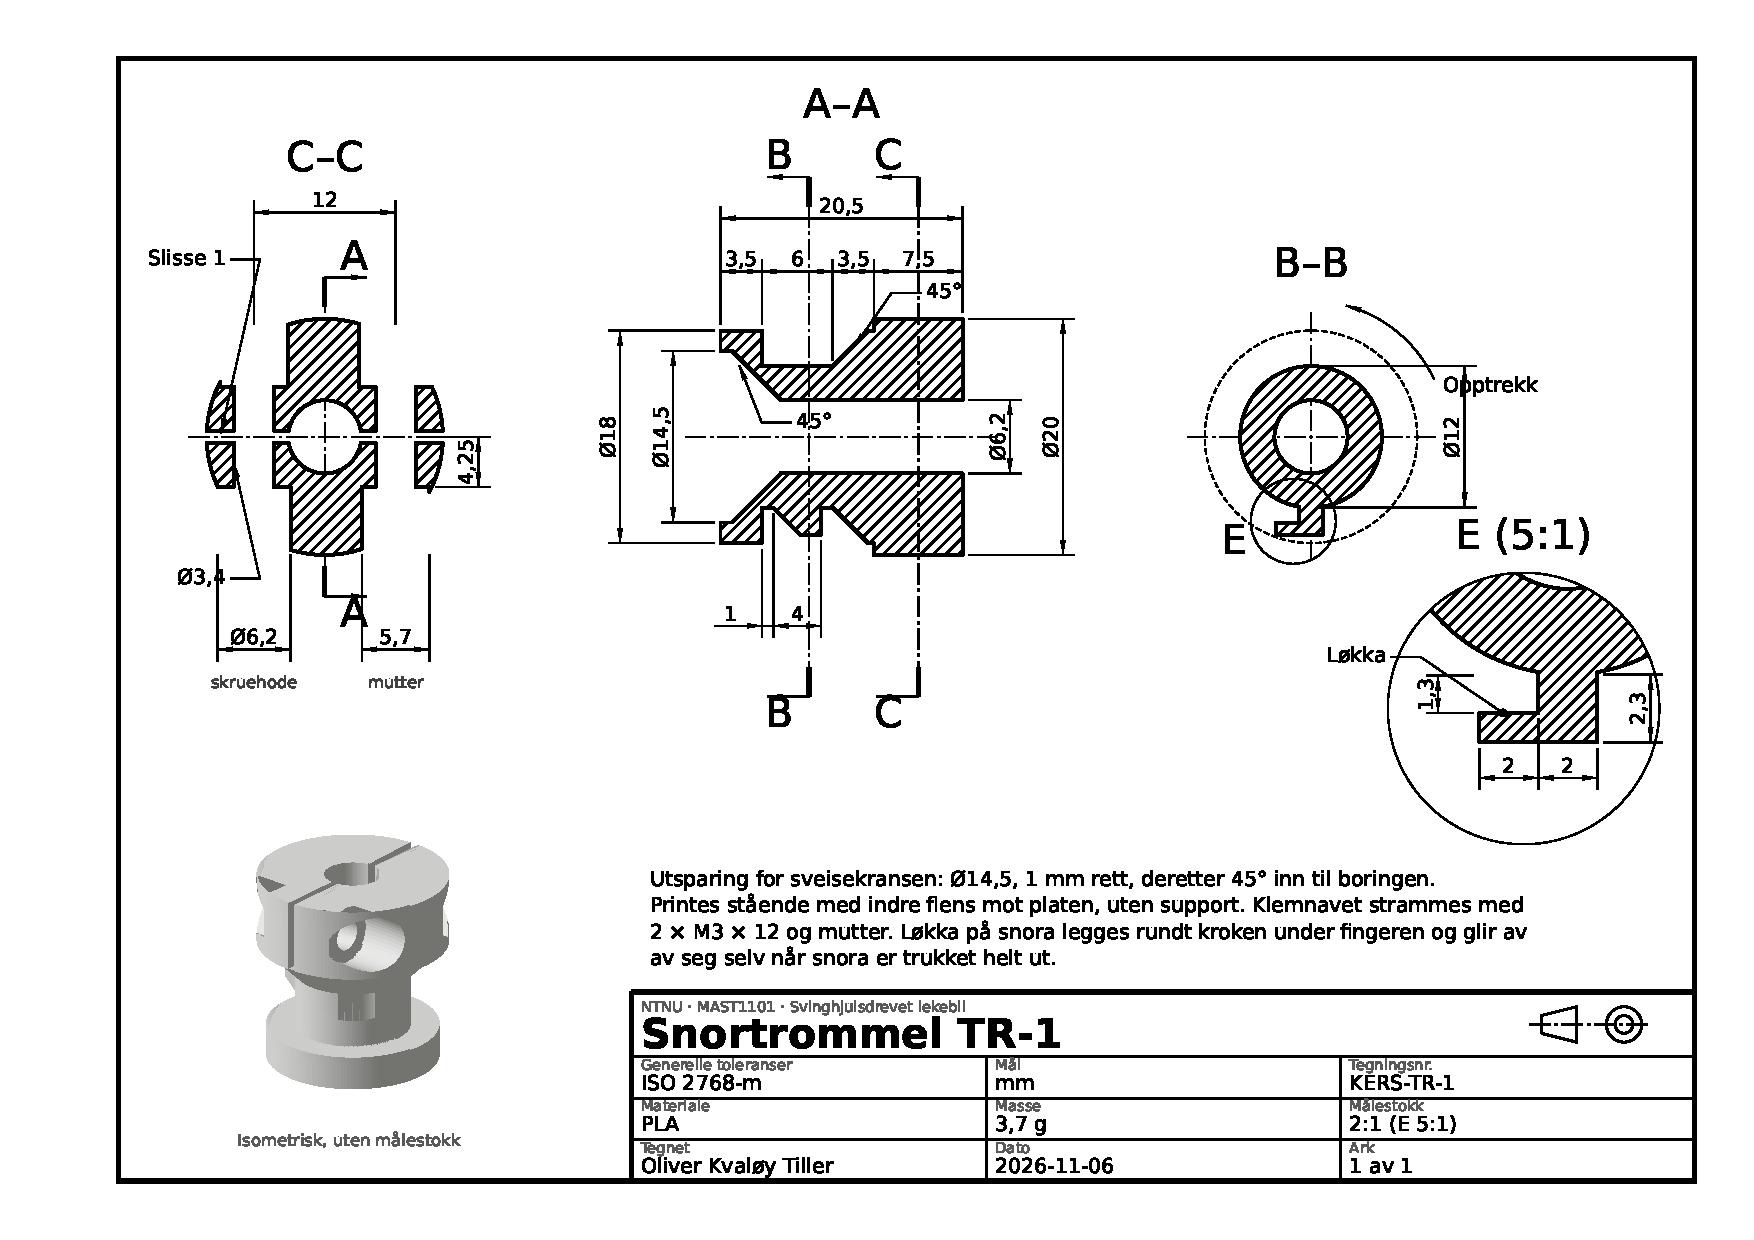
\includegraphics[width=\textheight]{Images/Tegninger/TR-1.pdf}
    \caption{Maskintegning av snortrommel TR-1. Snitt A--A langs aksen, C--C gjennom klemskruene, B--B gjennom kroken og detalj E av kroken.}
    \label{fig:snortrommel}
\end{sidewaysfigure}

Hovedtesten er turtallet etter opptrekk, målt med måleoppsettet i seksjon~\ref{sec:ml-serien}, med minst fem opptrekk per trommel. Snitt og standardavvik viser både turtall (R6) og repeterbarhet (R7). Tilleggstester er at snora løsner av seg selv fra trommelen ved enden av opptrekket, og at den ikke sklir av trommelen.

\begin{figure}[H]
    \centering
    \begin{subfigure}[b]{0.32\textwidth}
        \centering
        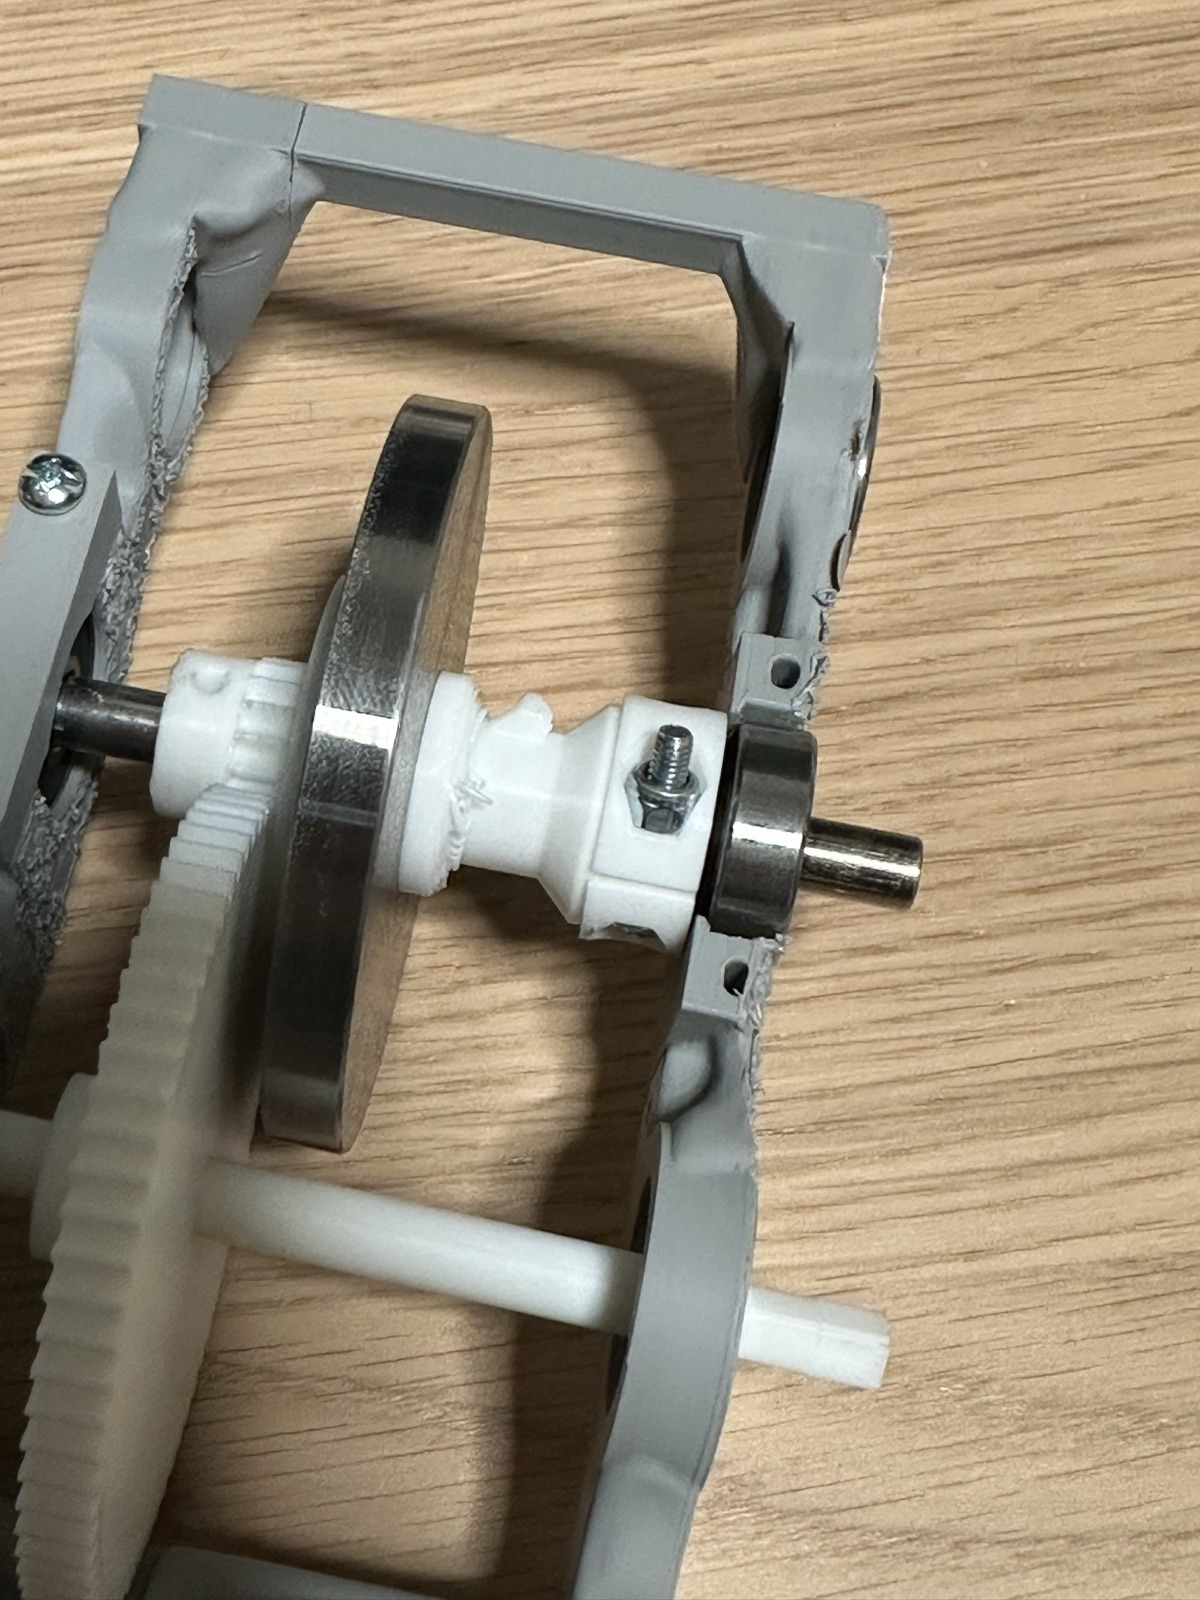
\includegraphics[width=\textwidth]{Images/Foto/trommel_klemnav.jpg}
        \caption{Klemnavet med de to M3-skruene}
    \end{subfigure}
    \hfill
    \begin{subfigure}[b]{0.32\textwidth}
        \centering
        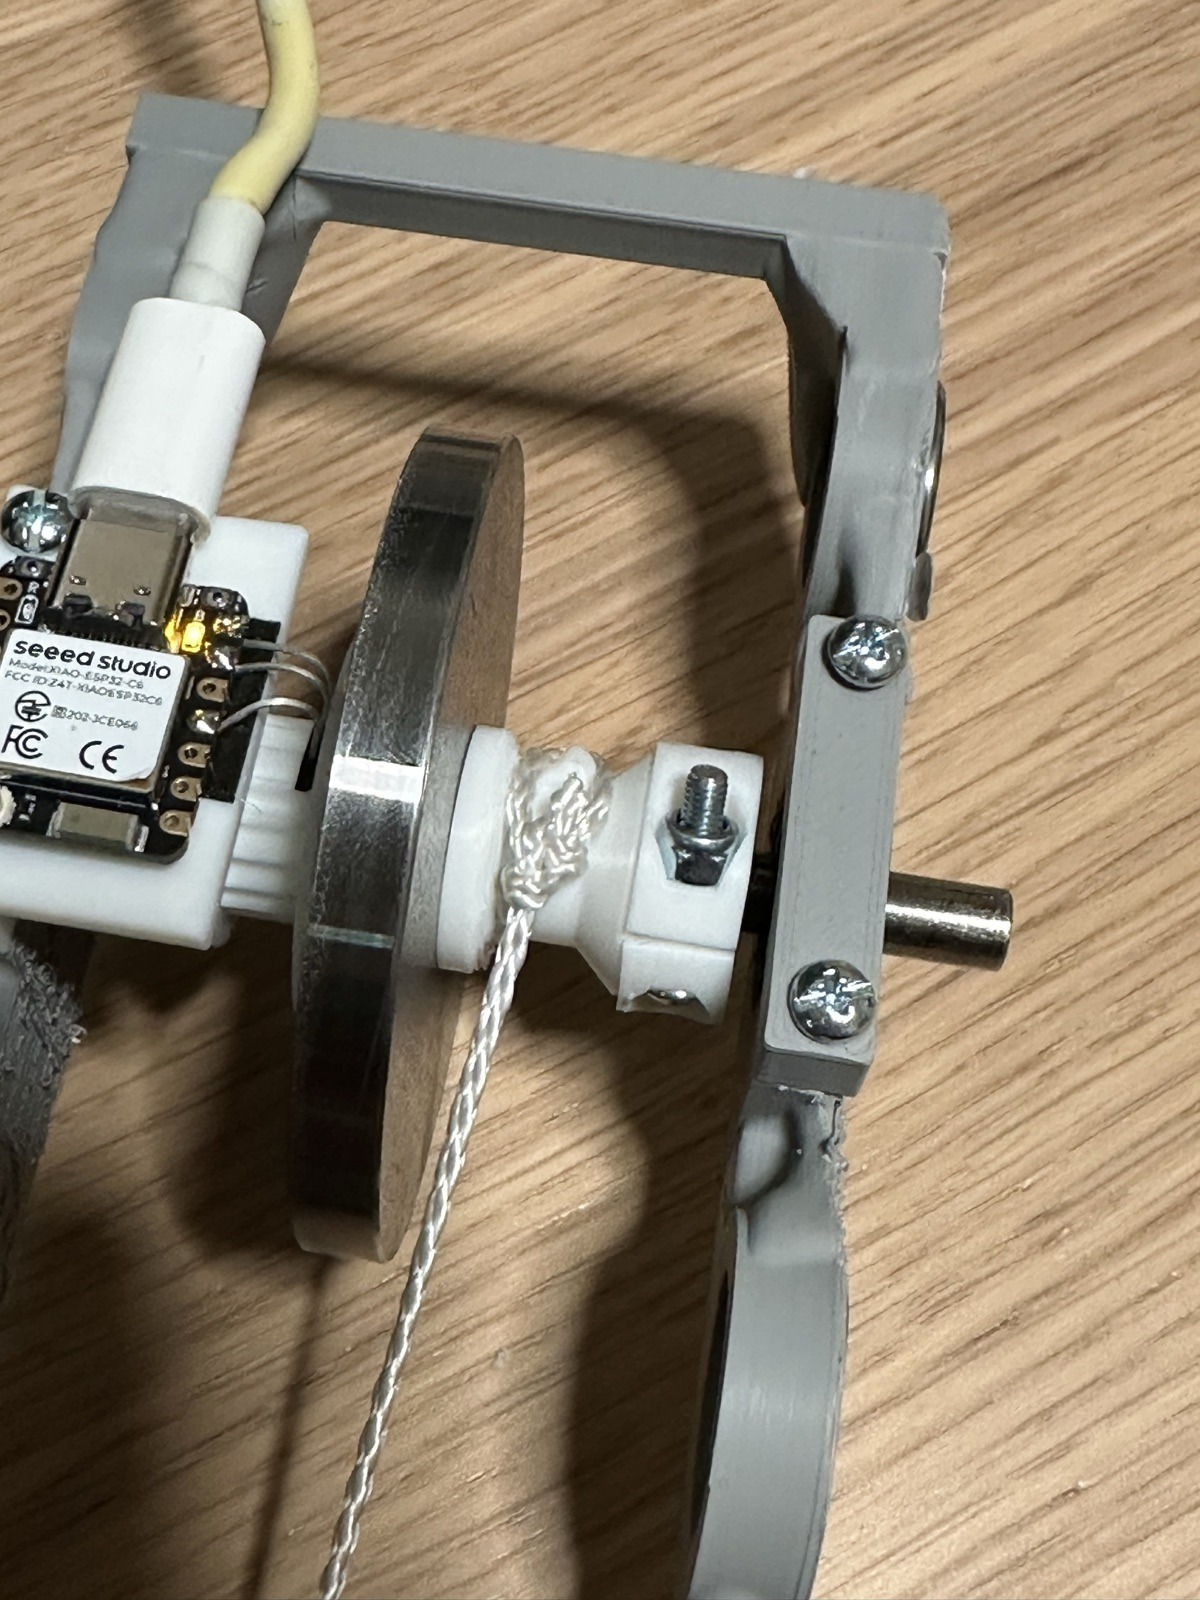
\includegraphics[width=\textwidth]{Images/Foto/trommel_snor.jpg}
        \caption{Snora viklet på trommelen}
    \end{subfigure}
    \hfill
    \begin{subfigure}[b]{0.32\textwidth}
        \centering
        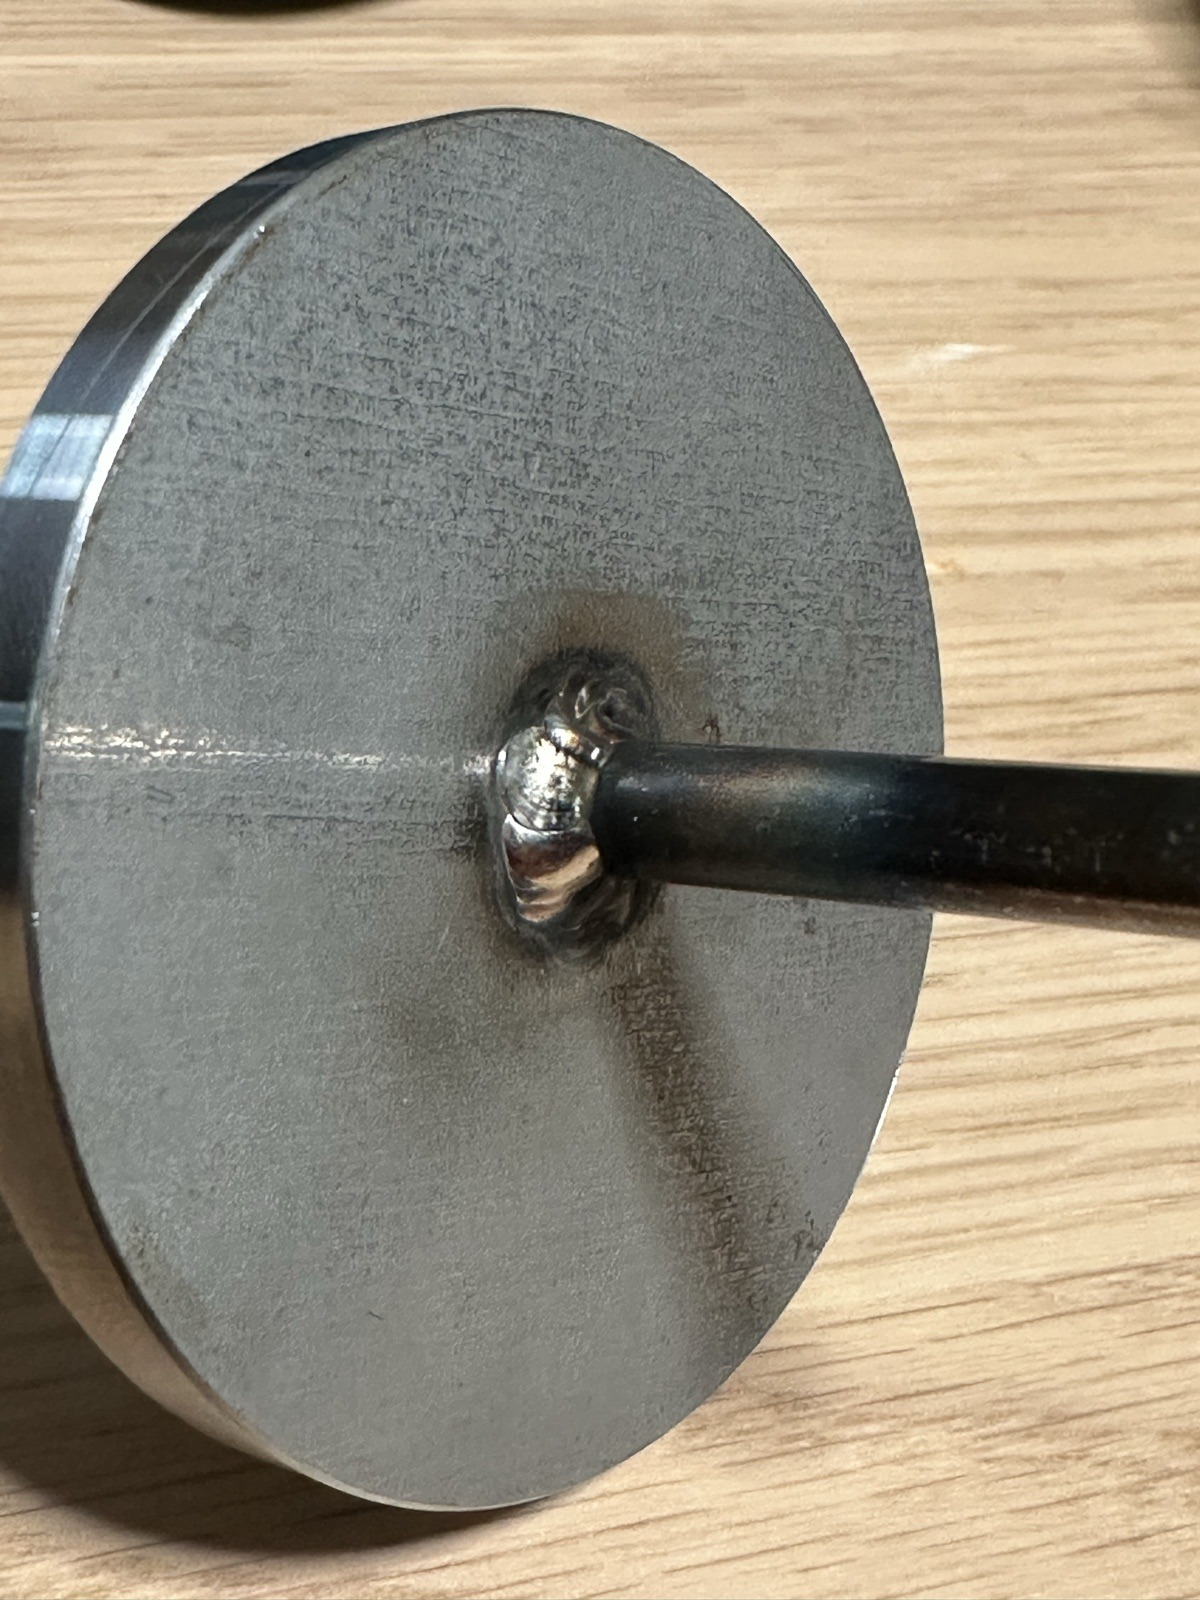
\includegraphics[width=\textwidth]{Images/Foto/svinghjul_sveis.jpg}
        \caption{Sveisekransen mellom svinghjul og aksel}
    \end{subfigure}
    \caption{TR-1 montert på svinghjulsakselen. Senkningen i den indre flensen gir plass til sveisekransen.}
    \label{fig:tr1-foto}
\end{figure}

De første opptrekkene er gjort med TR-1, som har den minste kjernen, $r_t = \SI{6}{mm}$.
Seks godkjente opptrekk ga \SI[separate-uncertainty=true]{2700 \pm 390}{o/min} rett etter at løkka slapp, med variasjonskoeffisient \SI{15}{\percent}. Det tilsvarer omtrent \SI{2,4}{J}, under halvparten av de \SI{5,3}{J} som simuleringen antok. I ett av åtte opptrekk hang løkka seg opp, og svinghjulet stoppet på under ett sekund. Rett etter at løkka slipper, bremses svinghjulet ekstra i omtrent \SI{0,3}{s}, som tyder på at løkka eller snora drar litt i trommelen før den er helt fri.

\begin{versjonstabell}{TR-1}{tab:tr1}
    \hovedtest
    Turtall etter opptrekk, \SI[separate-uncertainty=true]{2700 \pm 390}{o/min}, 6 opptrekk (R6, R7) & Delvis vellykket, under antatt \SI{4000}{o/min} \\
    \tilleggstester
    Snora løsner av seg selv & Delvis vellykket, hang seg opp i 1 av 8 \\
    Snora sklir ikke av trommelen & Vellykket \\
\end{versjonstabell}

\subsubsection{Drivhjul og dekk (DH)}
\label{sec:dh-serien}
Drivhjulene har ytre diameter \SI{68}{mm}, fastlagt i DV-3. Når bilen settes ned med svinghjulet i gang, slurer hjulene til farten passer med svinghjulet. Simuleringen viser at dekket påvirker distansen mest gjennom rullemotstanden. Halveres rullemotstandskoeffisienten fra 0,03 til 0,015, øker simulert distanse fra 38 til \SI{61}{m}, mens tre ganger så høy friksjonskoeffisient mot underlaget, fra 0,3 til 0,9, bare gir omtrent \SI{5}{\percent} lengre distanse. Et dekk bør derfor ha lav rullemotstand, og nok grep til at bilen går rett.

Alle hjulene har samme nav. Figur~\ref{fig:hjul} er maskintegningen av DH-2. Det har firkanthull fra NV-2 og en krage med diameter \SI{7,8}{mm} på innsiden. Kragen ligger an mot innerringen i lageret, aldri mot ytterringen, og holder akselen på plass sideveis. Seks eiker i en \SI{2}{mm} skive på utsiden holder massen og treghetsmomentet nede, og hjulet printes liggende med utsiden ned. Serien prøver tre hjul:
\begin{description}
    \item[DH-1: Bart hjul.] Hjulet i PLA uten dekk, med ytre diameter \SI{68}{mm}. Veier \SI{9,4}{g}.
    \item[DH-2: TPU-dekk.] En PLA-felg med sete på Ø65 og skuldre på begge sider, og et \SI{1,5}{mm} tykt dekk printet i TPU. Dekket har \SI{0,6}{mm} mindre indre diameter enn setet og strekkes over felgen. Ferdig diameter er \SI{68}{mm}, og felg og dekk veier til sammen \SI{8,8}{g}.
    \item[DH-3: TPU-dekk, Ø66.] Som DH-2, men \SI{2}{mm} mindre i diameter. Det gir \SI{2}{mm} margin til lengdekravet i R1 og \SI{1}{mm} lavere bakkeklaring.
\end{description}
Treghetsmomentet for fire hjul er $\SI{2,9e-5}{kg.m^2}$ for DH-2 og $\SI{2,6e-5}{kg.m^2}$ for DH-3, regnet fra CAD-geometrien. Det er omtrent halvparten av svinghjulets, men hjulene går $i$ ganger saktere, så bidraget til bilens effektive masse er lite.

\begin{figure}[H]
    \centering
    \begin{subfigure}[b]{0.36\textwidth}
        \centering
        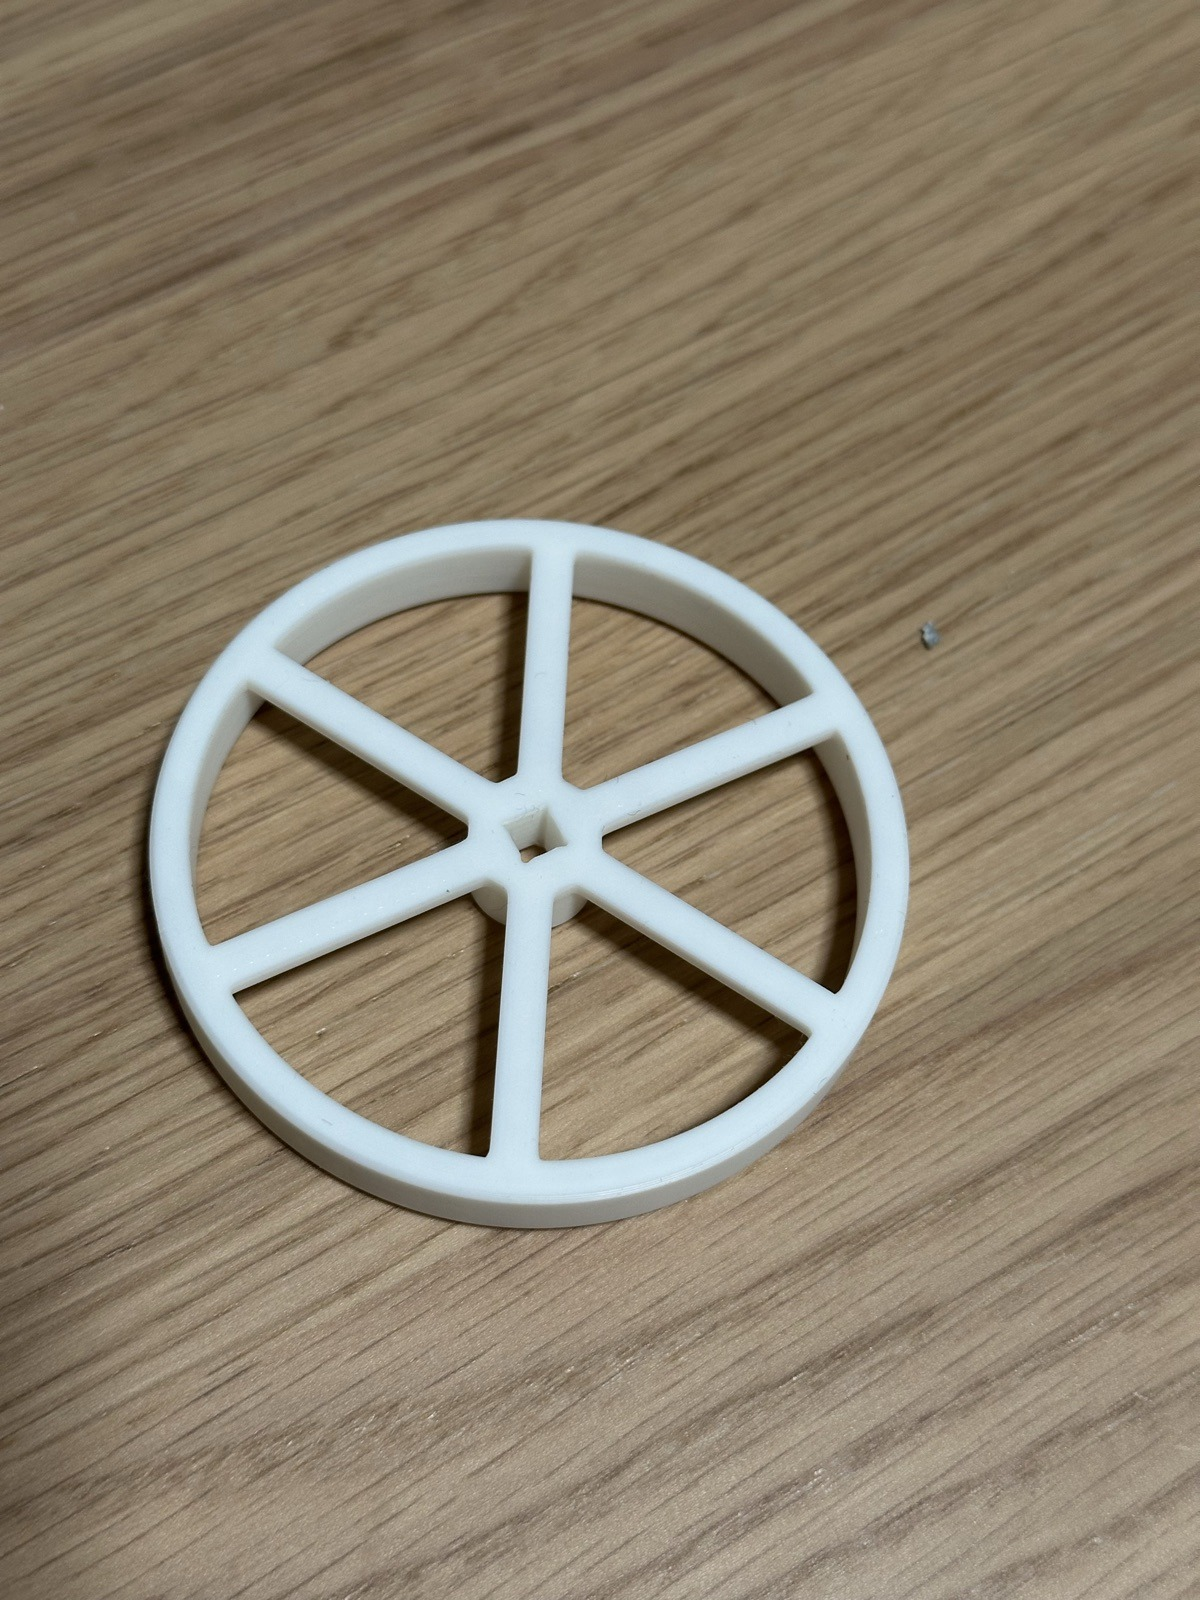
\includegraphics[width=\textwidth]{Images/Foto/felg_utside.jpg}
        \caption{Utsiden}
    \end{subfigure}
    \hspace{1.5em}
    \begin{subfigure}[b]{0.36\textwidth}
        \centering
        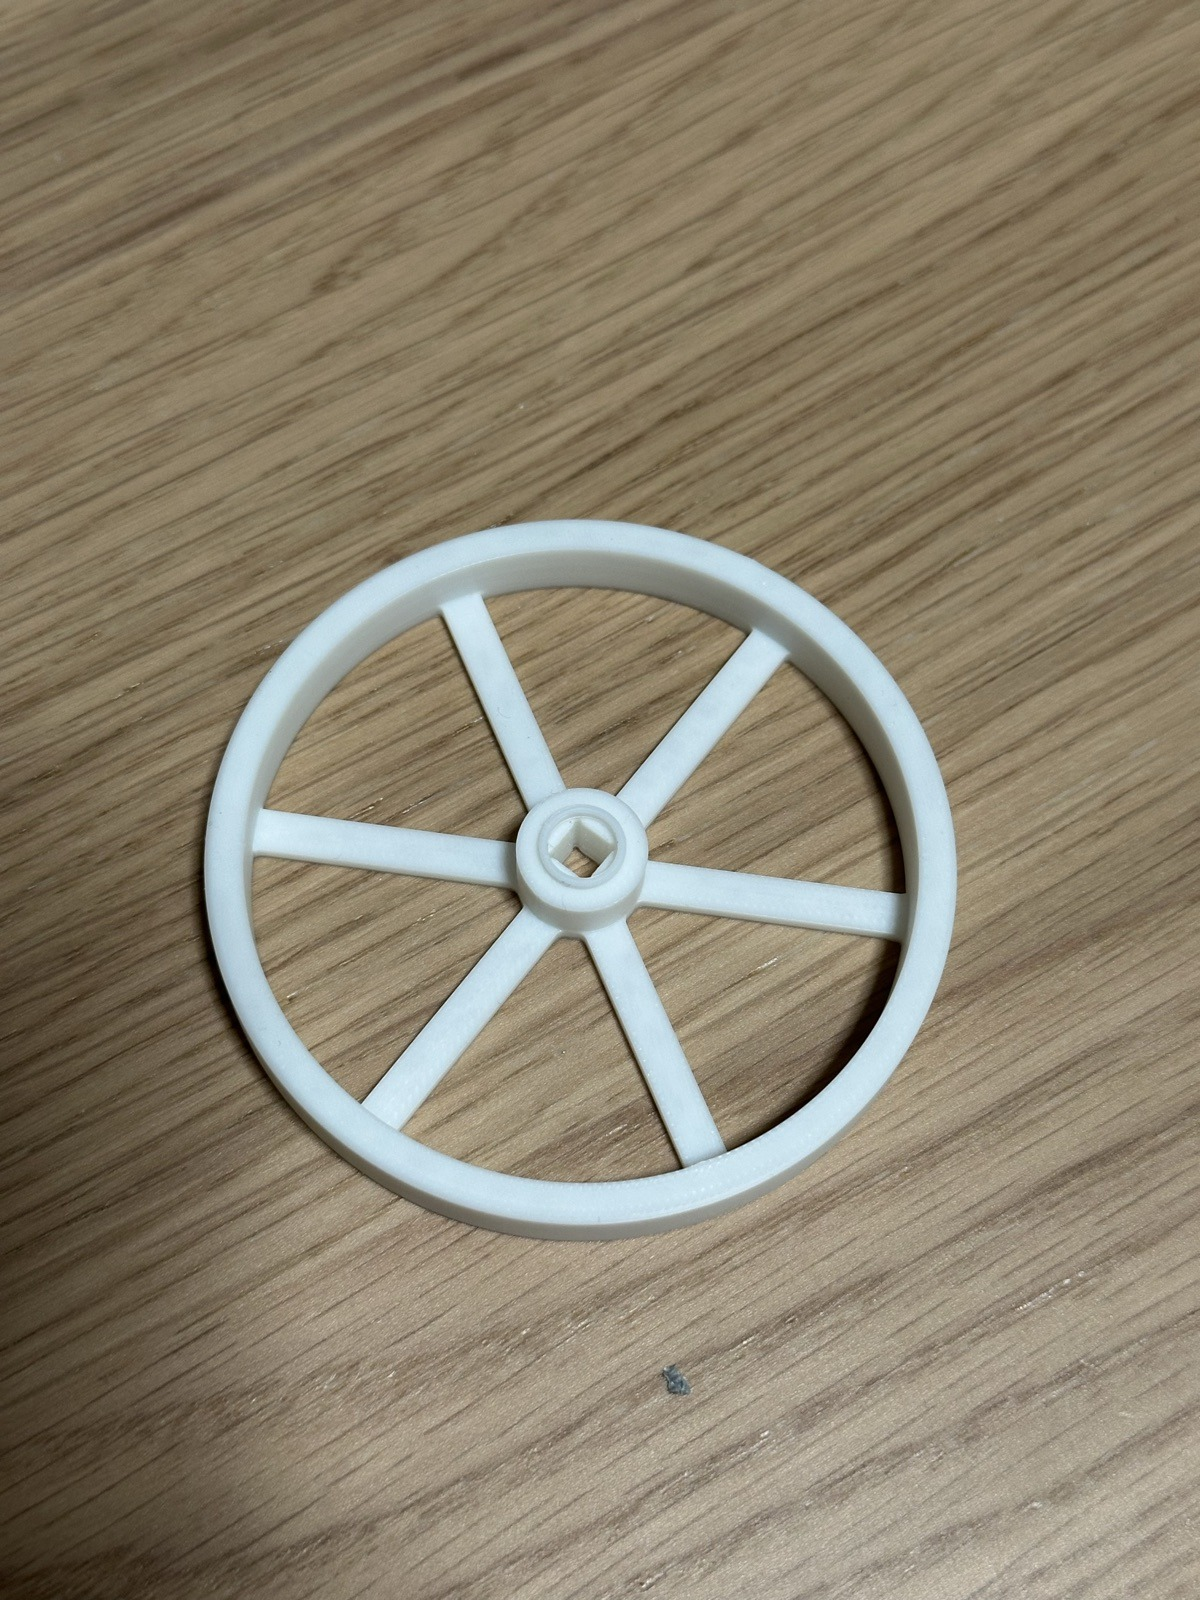
\includegraphics[width=\textwidth]{Images/Foto/felg_innside.jpg}
        \caption{Innsiden, med navet og kragen}
    \end{subfigure}
    \caption{Printet hjul fra DH-serien, uten TPU-dekk.}
    \label{fig:felg-foto}
\end{figure}

\begin{sidewaysfigure}
    \centering
    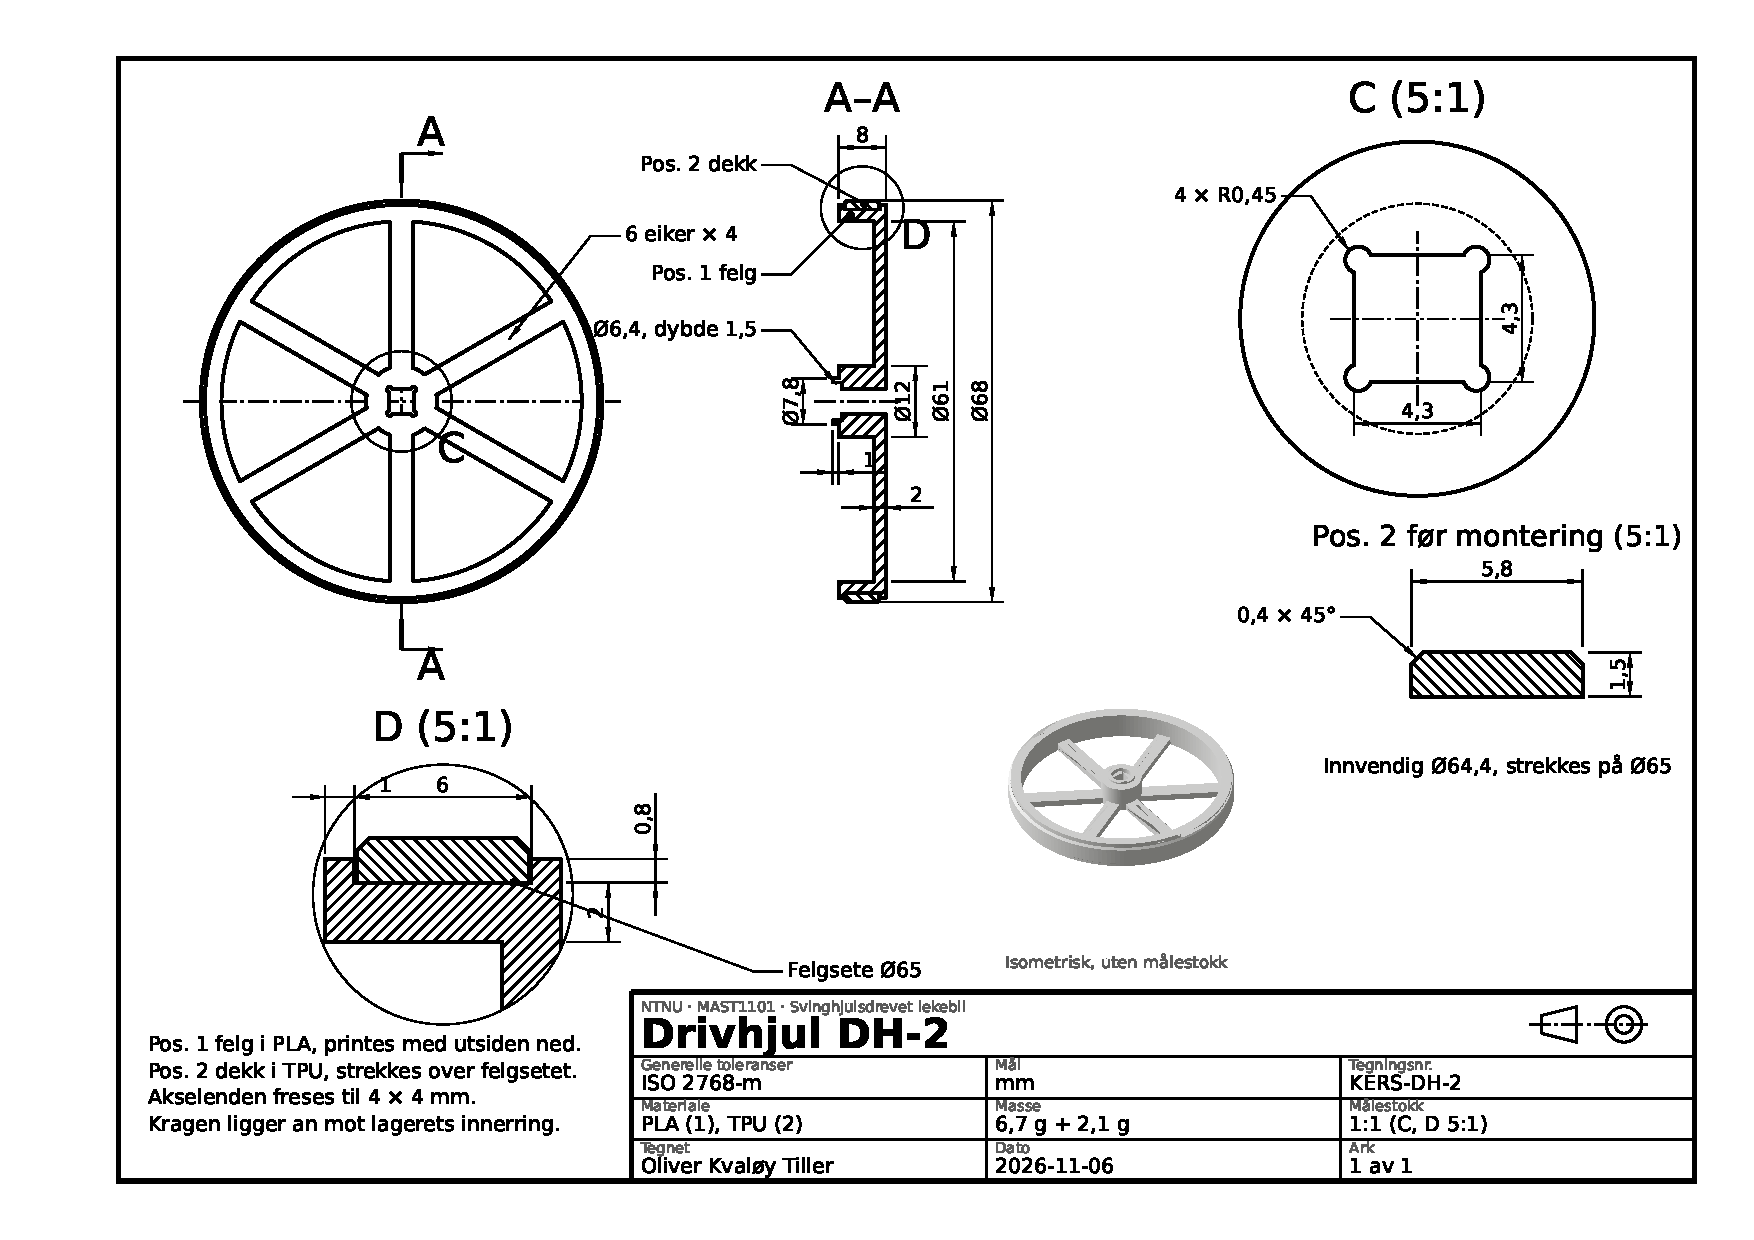
\includegraphics[width=\textheight]{Images/Tegninger/DH-2.pdf}
    \caption{Maskintegning av drivhjul DH-2 med felg (pos.~1) og TPU-dekk (pos.~2). DH-1 har samme nav og eiker, men er et bart hjul med ytre diameter \SI{68}{mm}.}
    \label{fig:hjul}
\end{sidewaysfigure}

Hovedtesten er kjøredistanse med minst 10 kjøringer per dekk (R6, R7). Tilleggstester er sideavvik (R8), at dekket sitter på hjulet gjennom hele testserien, og hvor lenge hjulene slurer ved nedsetting. Resultatene brukes også til å kontrollere rullemotstanden som er antatt i simuleringen.

\begin{comment}
\begin{versjonstabell}{DH-1}{tab:dh1}
    \hovedtest
    Kjøredistanse, snitt og standardavvik av 10 kjøringer (R6, R7) & \\
    \tilleggstester
    Sideavvik (R8) & \\
    Dekket sitter gjennom testserien & \\
    Slur ved nedsetting & \\
\end{versjonstabell}

% Samlet evaluering som tabell~\ref{tab:dv-samlet}, én tabell per serie når testene er gjort
\end{comment}

\begin{comment}
\subsubsection{Produksjonsmetoder og prosessvalg}
\subsubsection{Fremstilling og montering}
\subsubsection{Ferdig prototype og kontroll av dimensjoner}
% Beskriv materialer, produksjonsinnstillinger, monteringsprosedyre og kontrollmetoder. Vis bilder av den fremstilte prototypen. Skill mellom planlagt og utført arbeid.
\end{comment}

\subsection{Problemløsning}
\label{sec:problemlosning}
Testingen av den første prototypen avdekket fire problemer. Hvert av dem førte til en endring som er beskrevet i serien den hører til.

\paragraph{Sensoren så hver magnet tre ganger.} I ML-1 sto Hall-sensoren så nær magnetene at den også reagerte på feltet ved kanten av dem, og ga seks flanker per omdreining i stedet for to. Sensoren ble flyttet lenger unna, og loggeren ble endret til å registrere begge flankene (ML-2, seksjon~\ref{sec:ml-serien}).

\paragraph{Trommelen løsnet.} Klemnavet på trommelen sklei på akselen under den første serien. Det ble løst ved å kontrollere mutterne og stramme skruene jevnt (NV-1).

\paragraph{Svinghjulsakselen glir sideveis.} Med tannhjulet frakoblet varierte tapsmomentet fra 1,1 til \SI{2,0}{mN.m} mellom opptrekkene, mot \SI{3,6}{\percent} spredning med tannhjulet koblet (seksjon~\ref{sec:res-utsnurring}). Hvert opptrekk holdt et jevnt nivå hele veien ned, som tyder på at noe gnisset med ulik kraft fra gang til gang. Akselen hadde for mye klaring sideveis. Snora trekker litt på skrå, og avhengig av retningen kom trommelen borti rammen på den ene siden, eller pinjongen borti Hall-sensoren på den andre. Tiltaket er to avstandshylser som er laget, én mellom trommelnavet og lageret og én mellom magnetholderen og lageret på pinjongsiden (figur~\ref{fig:avstandshylse}). Hylsene er C-formede, med en \SI{5,3}{mm} åpning som er smalere enn akselen, så de klikkes på uten at akselen tas ut av lagrene. En krage med diameter \SI{7,8}{mm} ligger an mot innerringen i lageret, som roterer med akselen, så hylsene gir ingen ny friksjon. Lengden velges etter måling i trinn på \SI{0,5}{mm}, cirka 1,5 mm på trommelsiden og 5,0 til 5,5 mm på pinjongsiden, og klemnavene skyves inntil hylsene til akselen har 0,1 til \SI{0,3}{mm} klaring.

\begin{figure}[H]
    \centering
    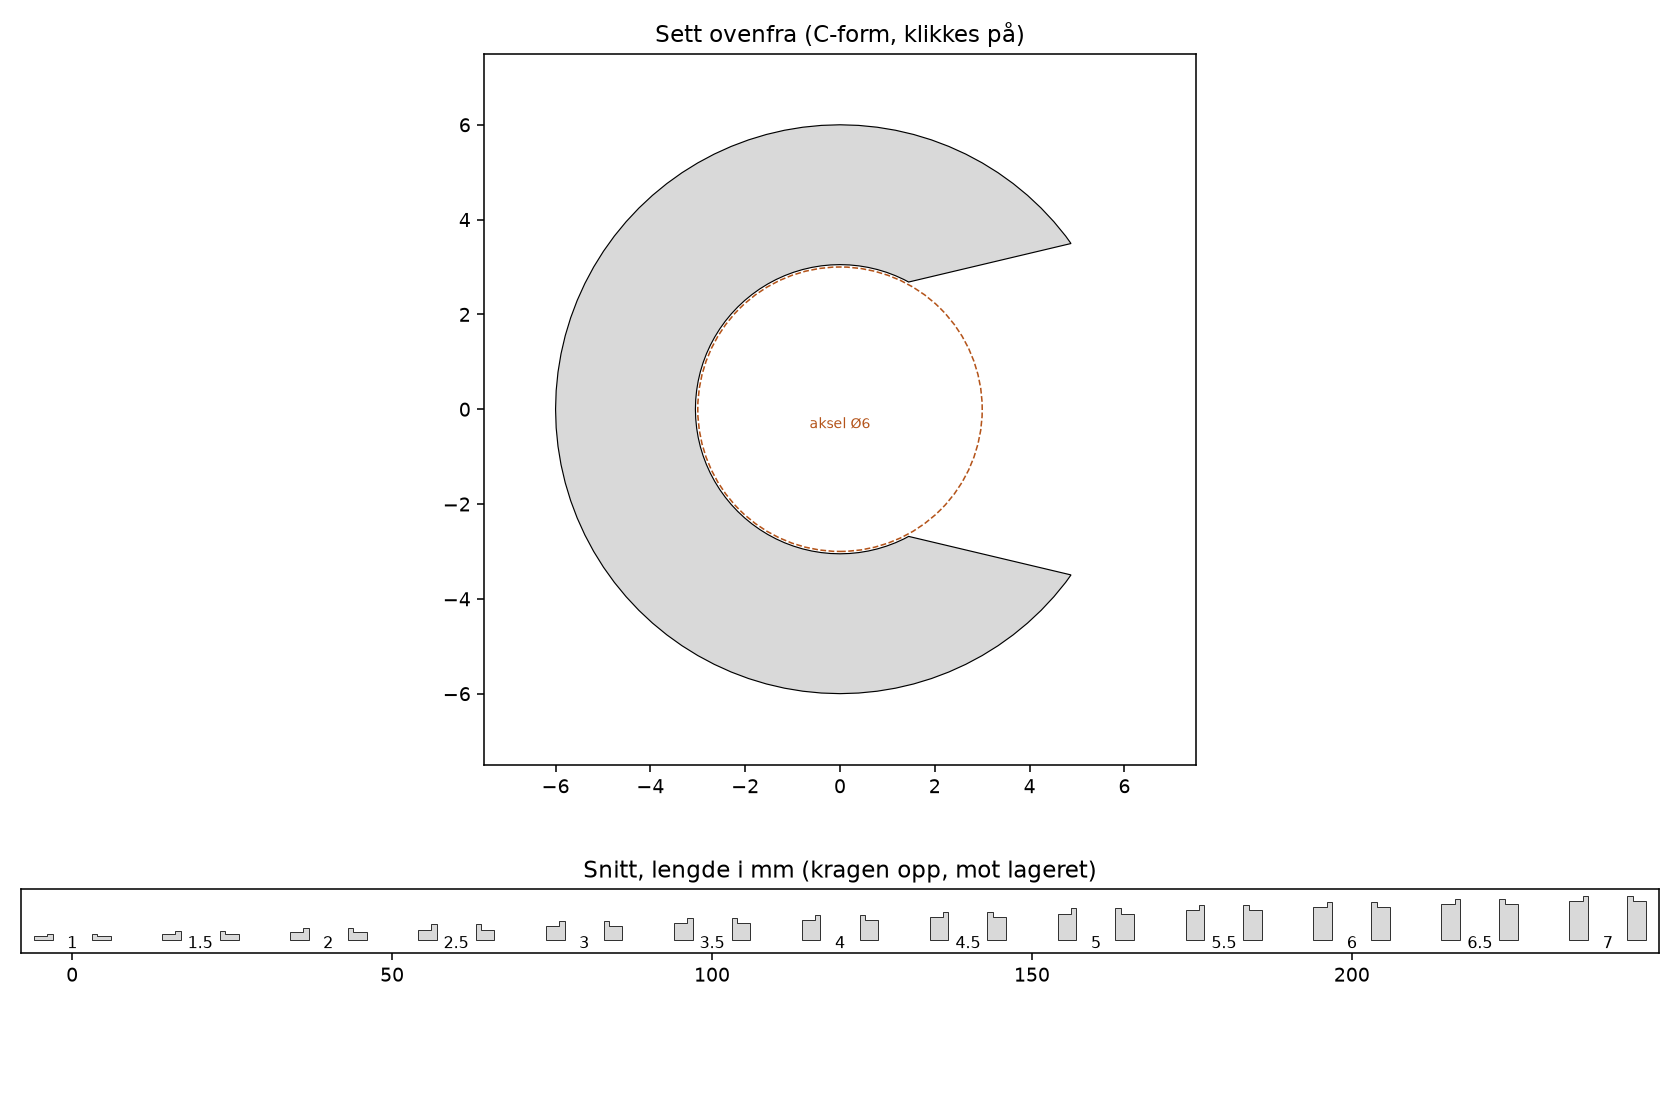
\includegraphics[width=0.7\textwidth]{Images/Prototyper/avstandshylse.png}
    \caption{Avstandshylse sett ovenfra, og snitt av settet med lengder fra 1,0 til \SI{7,0}{mm}.}
    \label{fig:avstandshylse}
\end{figure}

\paragraph{Fett i lagrene.} 626-lagrene leveres fylt med fett, som trolig står for en stor del av tapsmomentet som er målt. Planen er å ta ut tetningen på innsiden av hvert lager, vaske ut fettet med isopropanol, og smøre med én dråpe tynn olje. Lagrene skal ikke gå tørre, fordi de da ruster og slites. Den ytre tetningen beholdes, så det kommer mindre støv inn. Utsnurringen gjentas etterpå, slik at virkningen av tiltaket kan måles.
